\section{Histological Images Digitalization} \label{ssec:hist_im}
Modern histopathology is essentially based on the careful interpretation of microscopic images, with the intention of correctly diagnose patients and to guide therapeutic decisions. In the last years, thanks to the quick development of scanning techniques and image processing, the discipline of histology have seen radical improvements: the main of which undoubtedly is the passage from the microscope's oculars to the computer's screen. This digitalization process has brought several advantages, that were previously impossible in classical histology, like telepathology and remote assistance in diagnosis processes, the integration with other digitalized clinical workflows, and patients' history, and most importantly the opening to applications of artificial intelligence.
The name Whole Slide Imaging (WSI) refers to the modern virtual microscopy discipline, which consists of scanning a complete microscope slide and creating a single high-resolution digital file. This is commonly achieved by capturing many small high-resolution image tiles or strips and then montaging them to create a full image of a histological section. The four key steps of this process are image acquisition (scansion), editing, and on-screen image visualization.

In the field of Digital Pathology (DP) an essential concept in image understanding is the magnification factor, which indicates the scale of representation of the image and allows dimension referencing. This factor is usually indicated as the magnification power of the microscope's lenses used during the analysis. After the digitalization process, this original magnification factor is prone to change, depending on the resolution of the visualization screen. Therefore, image resolution is measured in $\mu m$ per pixel, and it is set by the different composition of the acquisition chain, as the optical sensor and the lenses. Histological scanner are usually equipped with 20$\times$ or 40$\times$ objectives, which correspond to 0.5 and 0.25 $mm$/pixels resolution values. Lenses with 20$\times$ magnification factor are the most suitable for the great majority of histopathological evaluations, and it is the golden standard for scansions, for its good trade-off between image quality and time of acquisition. Scansions with 40$\times$ magnification could increase four-fold acquisition and processing time, final file's dimension, and storage cost. A single WSI image, acquired with 20$\times$ will occupy more than 600 MB alone.

\begin{figure}
    \centering
    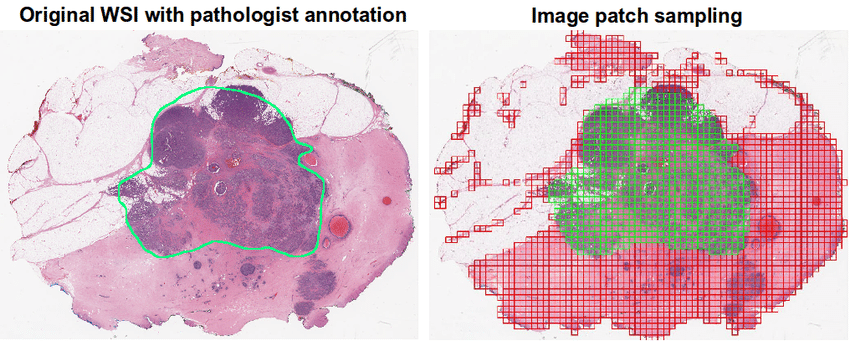
\includegraphics[width = \textwidth]{images/patches_grid}
    \caption{An example of whole slide image, with its grid decomposition in patches. It is visible the correspondence between a region of intereste maually anotated and the patches that matches that region. From \cite{WSI_grid}}
    \label{fig:patches_grid}
\end{figure}

Despite the WSI is a relatively mature discipline, it still struggles to integrate itself in the standard primitive diagnosis phase in histopathological laboratories. This is primarily due to some disadvantages, like images'resolution, image compression's artifacts, and auto-focusing algorithms, which plays a key role in the specimen interpretation. Furthermore, the scansion of histological samples is an additional step in the analysis which takes time. Despite the technological improvements the average time for the acquisition of a sample is around 5/10 minutes, depending on the number of slices in the slide, for just a single level of magnification. While in traditional histology, the pathologist has access to all the magnification levels at the same time. The real advantage, in fact, is in the long term. Once the images have been acquired they can be archived and consulted remotely almost instantaneously, helping clinical analysis and allowing remote assistance (telemedicine). Furthermore, the images now can be processed by artificial intelligence algorithms, allowing the application of technologies like Deep Learning which could revolutionize the research field, as already has been on many different disciplines in the scientific world.

In order to allow to automatically process, such big images as the ones obtained through WSI, it is necessary to subdivide them in smaller patches. The dimension of which should be big enough to allow interpretation and to preserve a certain degree of representability of the original image. In Figure \ref{fig:patches_grid} is shown an example of whole slide image, with its grid decomposition in patches. If the patches are too small, it should be over-specified for a particular region of tissue, loosing its general features. This could lead the learning algorithm to misinterpretation. However, this is not an exclusive limit of digital pathology, for a human pathologist would be impossible too to make solid decisions on a too limited sample of tissue. After the subdivision in patches, a typical process for biomedical images is the so-called \textit{data augmentation} of images, that is the process of creating re-newed images from the starting material through simple geometrical transformations, like translation, rotation, reflection, zoom in/out.

The analysis of histological images usually consists in detecting the different components in the samples and to recognise their arrangment as an healthy or pathological pattern. It is necessary to recognize every sign of vitality of the cells, evaluating the state of the nucleus. There are many addittional indicators to consider like the presence of inflammatory cells or tumoral cells. Furthermore, samples taken from different part of the human body present completely different characteristics, and this increase greatly the complexity of the analysis.
A reliable esamination of a sample thus require a careful inspection made by an high qualified expert. The automatization of this procedure would be extremily helpful, giving an increadible boost both in timing and in accessibility. However, this is not a simple task and in section \ref{ssec:soa_seg} I will show some actual model for biomedical image processing in detail.

 \begin{figure}
     \centering
     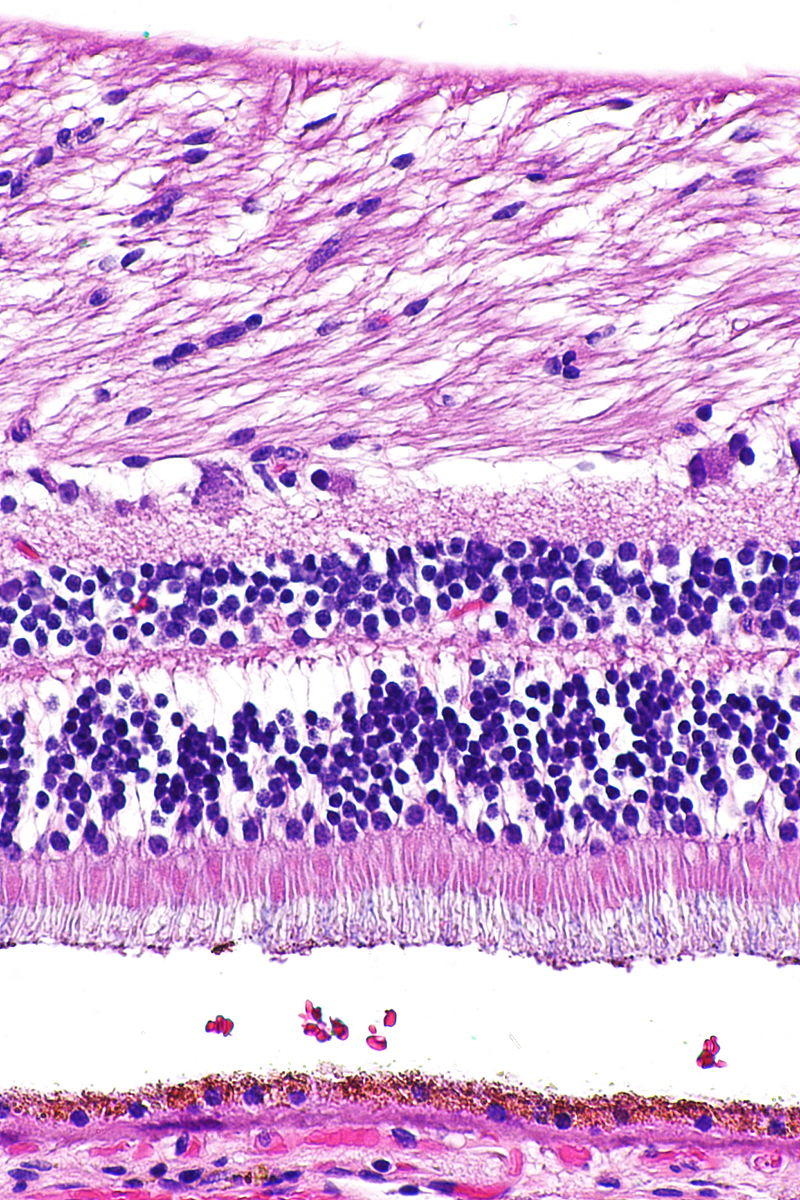
\includegraphics[width = 0.3\textwidth]{images/h&e_retyna}
     \caption{A sample of tissue from a retina (a part of the eye) stained with hematoxylin and eosin, cell nuclei stained blue-purple and extracellular material stained pink.}
     \label{fig:he_retyna}
 \end{figure}

\subsection{Slides Preparation for Optic Microscopic Observation} \label{ssec:samp_prep}
In modern, as in traditional, histology regardless on the final support of the image the slide has to be physically prepared, starting from the sample of tissue. The sample and slide preparation is a crucial step for histological or cytological observation. It is essential to highlight what needs to be observed and to \textit{immobilize} the sample at a particular point in time and with characteristics close to those of its living state. There are five key steps for the preparation of samples \cite{Alturkistani2015}:
\begin{description}
    \item [1) Fixation] is carried out immediately after the removal of the sample to be observed. It is used to immobilize and preserve the sample permanently in as life-like state as possible. It can be performed immersing the biological material in a formalin solution or by freezing, so immersing the sample in a tissue freezing medium which is then cooled in liquid nitrogen.

    \item [2) Embedding] if the sample has been stabilazed in a fixative solution, this is the subsequent step. It consists in hardening the sample in a paraffin embedding medium, in order to be able to carry out the sectioning. It is necessary to dehydrate the sample beforehand, by replacing the water molecules in the sample with ethanol.

    \item [3) Sectioning] Sectioning is performed using microtomy or cryotomy. Sectioning is an important step for the preparation of slides as it ensures a proper observation of the sample by microscopy. Paraffin-embedded samples are cut by cross section, using a microtome, into thin slices of 5 $\mu m$. Frozen samples are cut using a cryostat. The frozen sections are then placed on a glass slide for storage at -80$\degree$C. The choice of these preparation conditions is crucial in order to minimize the artifacts. Paraffin embedding is favored for preserving tissues; freezing is more suitable for preserving DNA and RNA and for the labeling of water-soluble elements or of those sensitive to the fixation medium.

    \item [4) Staining] Staining increases contrasts in order to recognize and differentiate the different components of the biological material. The sample is first deparaffinized and rehydrated so that polar dyes can impregnate the tissues. The different dyes can thus interact with the components to be stained according to their affinities. Once staining is completed, the slide is rinsed and dehydrated for the mounting step.

\end{description}

Hematoxylin and eosin stain (H\&E) is one of the principal tissue stains used in histology \cite{he_stain}, and it is the most widely used stain in medical diagnosis and is often the gold standard \cite{Rosai2007}. H\&E is the combination of two histological stains: hematoxylin and eosin. The hematoxylin stains cell nuclei blue, and eosin stains the extracellular matrix and cytoplasm pink, with other structures taking on different shades, hues, and combinations of these colors. An example of H\&E stained is shown in Figure \ref{fig:he_retyna}, in which we can see the typical colour palette of an histological specimen.
